\subsubsection{Barren Plateaus}\label{sec:barren-plateaus}

The Barren Plateau is a fundamental challenge in Variational Quantum Algorithms (VQAs), and the idea is very intuitive once we understand what a gradient represents.

\highspace
\begin{flushleft}
    \textcolor{Green3}{\faIcon{question-circle} \textbf{What is a Gradient?}}
\end{flushleft}
Suppose we have a \textbf{cost function} $C(\theta)$ where $\theta$ is one \textbf{parameter} of the Ansatz. The optimizer wants to know: ``\emph{\textbf{if I change $\theta$ slightly, will the cost improve?}}''. The answer is given by the \textbf{gradient}:
\begin{equation*}
    \frac{\partial C}{\partial \theta}
\end{equation*}
Because the gradient measures \textbf{how sensitive the cost function is to\break changes in the parameters}, it tells the optimizer which direction to move $\theta$ to improve the cost.

\highspace
\textcolor{Green3}{\faIcon[regular]{lightbulb}} Imagine we are hiking on a mountain. The slope tells us \emph{which} direction is downhill and \emph{how} steep the terrain is. The optimizer uses the gradient in exactly the same way.
\begin{itemize}
    \item If the \textbf{gradient} is \textbf{large}, the optimizer knows that a small change in $\theta$ will lead to a significant improvement in the cost function (i.e., the cost will \hl{decrease quickly}).
    \item If the \textbf{gradient} is \textbf{small}, the optimizer cannot determine whether changing $\theta$ will improve the cost function, as the change will be negligible.
\end{itemize}

\highspace
\begin{flushleft}
    \textcolor{Green3}{\faIcon{question-circle} \textbf{What is a Barren Plateau?}}
\end{flushleft}
Suppose our ansatz has \textbf{only one parameter} $\theta$. For every value of $\theta$, we can compute $C\left(\theta\right)$. For example:

\begin{center}
    \begin{tabular}{@{} c c @{}}
        \toprule
        $\theta$ & Cost \\
        \midrule
        0.0 & 7.76 \\
        0.5 & 5.98 \\
        1.0 & 3.66 \\
        1.5 & 2.70 \\
        2.0 & 2.56 \\
        2.5 & 1.79 \\
        3.0 & 2.15 \\
        3.5 & 3.61 \\
        4.0 & 4.44 \\
        \bottomrule
    \end{tabular}
\end{center}

\noindent
If we plot the cost function, the optimizer likes this because it immediately sees ``\emph{go to the right, the cost decreases}''. The slope (gradient) is large.

\newpage

\begin{figure}[!htp]
    \centering
    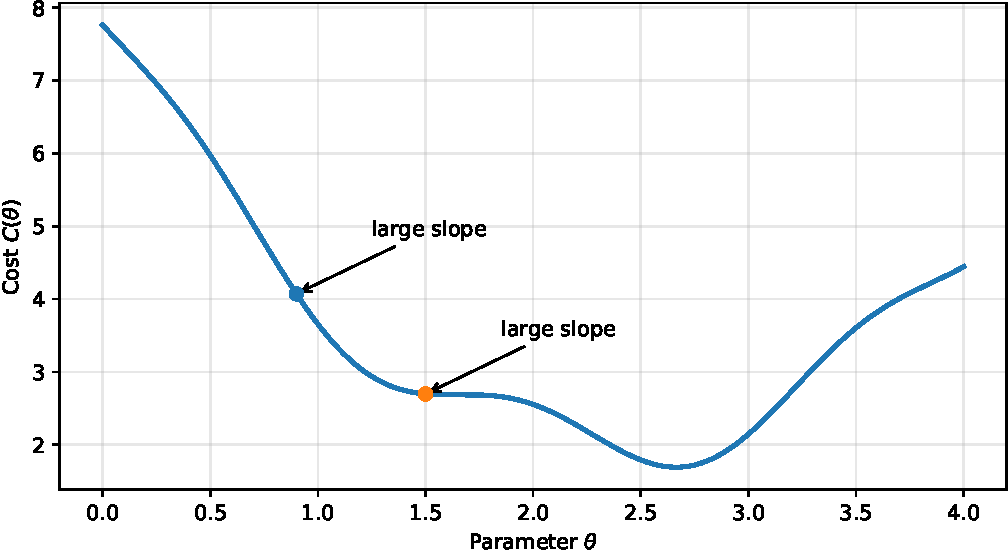
\includegraphics[width=\textwidth]{img/informative_landscape.pdf}
    % cost = (theta - 2.4) ** 2 + 0.4 * np.sin(4 * theta) + 2
    \caption{A cost function with a large gradient. The optimizer can easily determine which direction to move $\theta$ to improve the cost.}
\end{figure}

\noindent
Now suppose the cost values are:

\begin{center}
    \begin{tabular}{@{} c c @{}}
        \toprule
        $\theta$ & Cost \\
        \midrule
        % cost_flat = 5 + 0.001 * np.sin(8 * theta)
        % [(0.0, np.float64(5.0)), (0.5, np.float64(4.9992431975046925)), (1.0, np.float64(5.000989358246623)), (1.5, np.float64(4.9994634270819995)), (2.0, np.float64(4.999712096683335)), (2.5, np.float64(5.000912945250728)), (3.0, np.float64(4.999094421637993)), (3.5, np.float64(5.000270905788308)), (4.0, np.float64(5.000551426681242))]
        0.0 & 5.00 \\
        0.5 & 4.9992431975046925 \\
        1.0 & 5.000989358246623 \\
        1.5 & 4.9994634270819995 \\
        % 2.0 & 4.999712096683335 \\
        % 2.5 & 5.000912945250728 \\
        % 3.0 & 4.999094421637993 \\
        $\vdots$ & $\vdots$ \\
        \bottomrule
    \end{tabular}
\end{center}

\begin{figure}[!htp]
    \centering
    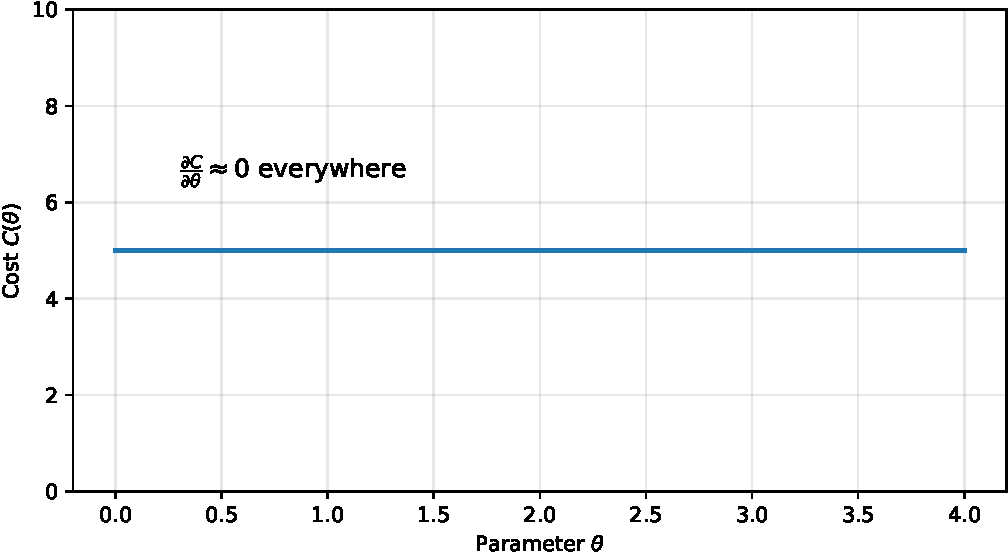
\includegraphics[width=\textwidth]{img/barren_plateau_flat.pdf}
    \caption{A cost function with a small gradient. The optimizer cannot determine which direction to move $\theta$ to improve the cost.}
\end{figure}

\noindent
Everything is almost identical. The optimizer asks: ``\emph{if I increase $\theta$, do I improve?}''. The answer is: ``\emph{I have no idea}''. The optimizer is \textbf{stuck}. This is a \textbf{barren plateau}!

\highspace
The gradient is simply $\frac{\partial C}{\partial \theta}$, and it tells us ``\emph{\textbf{how much does the cost change if we slightly change $\theta$?}}''. For large gradients, the optimizer can easily determine which direction to move $\theta$ to improve the cost. For small gradients, the optimizer cannot determine which direction to move $\theta$ to improve the cost.

\highspace
It is called \textbf{barren plateau} because the cost landscape is almost perfectly flat, like a desert. The optimizer is like a hiker trying to find the lowest point in an endless flat desert. Similarly, ``barren'' refers to the fact that there is \textbf{nothing useful} in the landscape to guide the optimizer.

\highspace
\textcolor{Green3}{\faIcon{book} \textbf{A more realistic picture.}} Actually, the landscape \textbf{is not perfectly flat}. There are small hills and valleys, but they are so small that the optimizer cannot distinguish them from numerical noise:
\begin{equation*}
    \frac{\partial C}{\partial \theta} \approx 0
\end{equation*}

\begin{figure}[!htp]
    \centering
    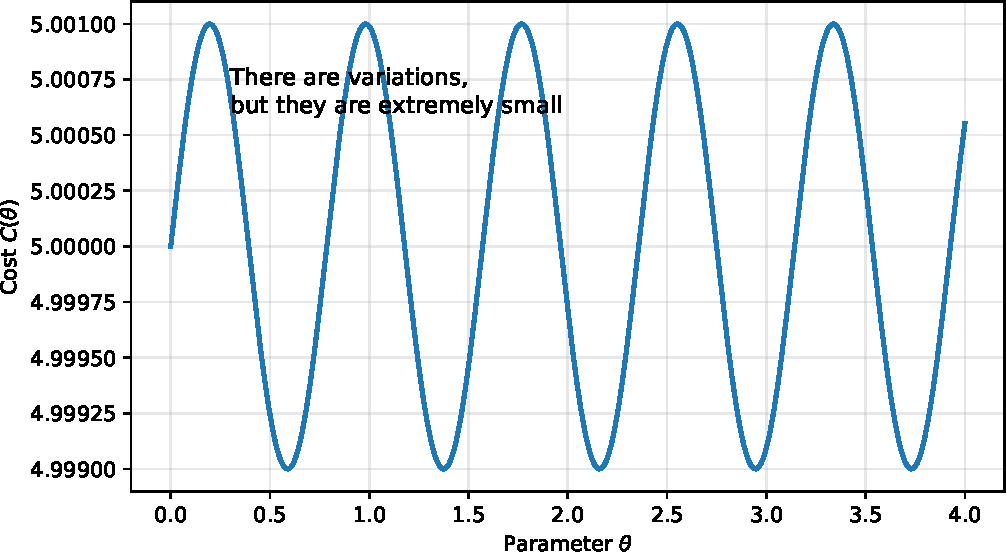
\includegraphics[width=\textwidth]{img/barren_plateau_zoom.pdf}
    \caption{A barren plateau is not perfectly flat. There are small hills and valleys, but they are so small that the optimizer cannot distinguish them from numerical noise.}
\end{figure}

\highspace
\textcolor{Green3}{\faIcon{bookmark} \textbf{Even more realistic: many parameters.}} In reality, the ansatz has \textbf{many} parameters:
\begin{equation*}
    \theta = (\theta_1, \theta_2, \ldots, \theta_n)
\end{equation*}
So the cost function is not a 2D curve $C\left(\theta\right)$, it is a surface in a very high-dimensional space $C\left(\theta_1, \theta_2, \ldots, \theta_n\right)$. In this case, a barren plateau becomes almost a \textbf{flat table}; th optimizer is trying to find the lowest point on that table, but every direction looks almost identical. In essence, \hl{a barren plateau is \textbf{not a property of the optimizer}, it is a \textbf{property of the cost function landscape}.}

\begin{figure}[!htp]
    \centering
    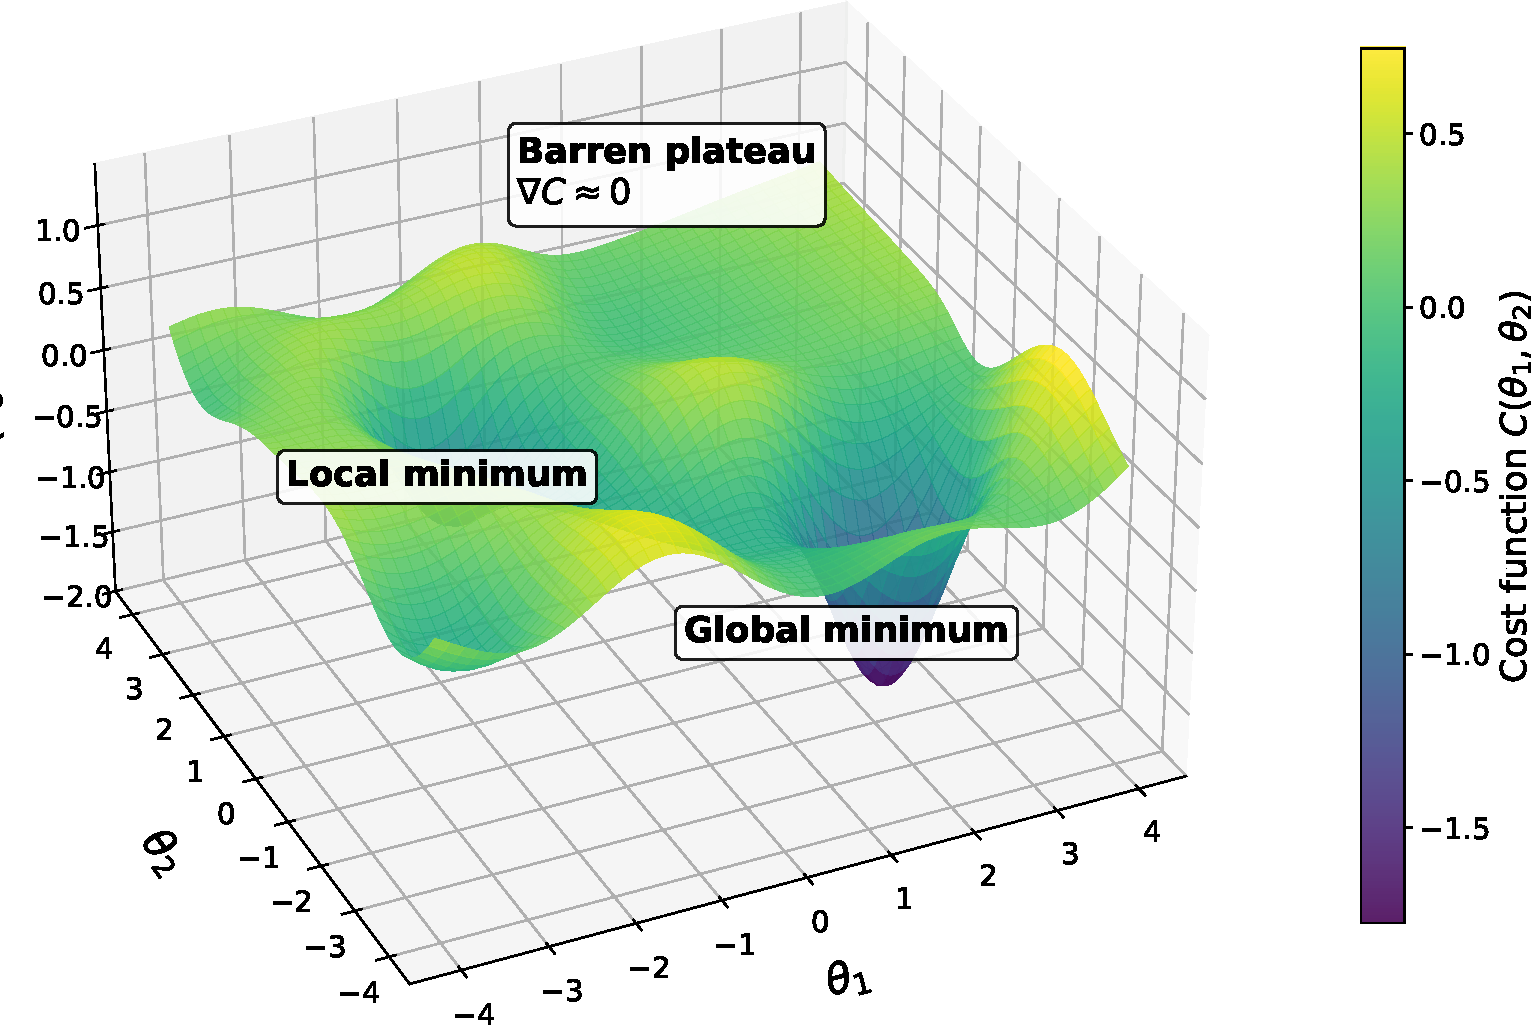
\includegraphics[width=\textwidth]{img/barren-plateau.pdf}
\end{figure}

\begin{flushleft}
    \textcolor{Green3}{\faIcon{question-circle} \textbf{Why do Barren Plateaus occur?}}
\end{flushleft}
We have seen what a barren plateau is, but we have not yet explained \textbf{why} they occur. Let's try to understand the reason behind this phenomenon.
\begin{itemize}
    \item \important{What is the optimizer trying to do?} The optimizer is trying to minimize:
    \begin{equation*}
        C\left(\theta\right) = \bra{\psi(\theta)} H \ket{\psi(\theta)}
    \end{equation*}
    Where $C\left(\theta\right)$ is the cost function, and $\bra{\psi(\theta)} H \ket{\psi(\theta)}$ is the \textbf{expectation value} of the Hamiltonian $H$ with respect to the quantum state $\ket{\psi(\theta)}$. In other words, it answers the question: \hl{``\emph{if our system is in the state $\ket{\psi(\theta)}$, what energy should we expect to measure?}''}. It is simply the average energy of the system in that state.

    \begin{examplebox}[: Expectation Value]
        For example, suppose our state $\ket{\psi(\theta)}$ is 50\% ground state $\ket{\psi_{0}}$ and 50\% first excited state $\ket{\psi_1}$. Then the expected energy is:
        \begin{equation*}
            0.5 E_0 + 0.5 E_1
        \end{equation*}
        Where $E_0$ is the energy of the ground state and $E_1$ is the energy of the first excited state. The expectation value:
        \begin{equation*}
            \bra{\psi(\theta)} H \ket{\psi(\theta)} = 0.5 E_0 + 0.5 E_1
        \end{equation*}
        It is literally a \textbf{weighted average} of the energies.
    \end{examplebox}

    The Hamiltonian $H$ assigns an energy to every possible quantum state. Then, the Ansatz circuit generates candidate states $\ket{\psi(\theta)}$ by varying the parameters $\theta$. Finally, the optimizer tries to find the parameters $\theta$ that minimize the expected energy. The optimizer is trying to find the \textbf{ground state} of the Hamiltonian $H$ (i.e., the state with the lowest energy $E_0$). So the Hamiltonian acts almost like a \textbf{judge}, the ansatz proposes every state with an energy, and the optimizer tries to find the state with the lowest energy.

    \highspace
    Geometrically, the optimizer is trying to find the \textbf{lowest point} in a very high-dimensional landscape. The landscape is defined by the cost function $C\left(\theta\right)$, which assigns a height (energy) to every point (parameter configuration) in the landscape. To \textbf{reach the lowest point}, the optimizer needs to know which direction to move in the landscape. The \hl{gradient is the only information that tells the optimizer which direction to move}:
    \begin{equation*}
        \nabla C\left(\theta\right) = \left(\frac{\partial C}{\partial \theta_1}, \frac{\partial C}{\partial \theta_2}, \ldots, \frac{\partial C}{\partial \theta_n}\right)
    \end{equation*}
    For each parameter $\theta_i$, the gradient tells the optimizer how much the cost function changes if we slightly change $\theta_i$. After computing the gradient, the optimizer updates the parameters $\theta$ in the direction of the negative gradient to decrease the cost function. We do not present the details of the optimization algorithm here, but the key point is that \textbf{the optimizer relies on the gradient to find the lowest point in the landscape}.


    \item \important{Add more parameters and many qubits}. Imagine 20 qubits and 100 parameters. The optimizer is trying to find the \textbf{lowest point in a 100-dimensional landscape}. The gradient is a vector with 100 components, and each component tells the optimizer how much the cost function changes if we slightly change one of the parameters. As we increase the number of qubits, the number of parameters increases, and the \textbf{landscape becomes more complex}. The optimizer has to explore a larger space, and it becomes more likely that it will encounter regions where the gradient is very small.
    

    \item \important{Averaging effect}. Since the cost function tries to minimize the expectation value of the Hamiltonian:
    \begin{equation*}
        C\left(\theta\right) = \bra{\psi(\theta)} H \ket{\psi(\theta)}
    \end{equation*}
    The optimizer is effectively averaging over many possible states. As the number of qubits increases, the number of possible states grows exponentially. Many positive and negative contributions to the gradient cancel each other out, leading to a very small overall gradient. This is known as the \textbf{averaging effect}, and it is a key reason why barren plateaus occur.

    \begin{examplebox}[: Averaging Effect]
        For example, consider a simple case where the Hamiltonian has two terms:
        \begin{equation*}
            H = H_1 + H_2
        \end{equation*}
        The cost function is:
        \begin{equation*}
            C\left(\theta\right) = \bra{\psi(\theta)} H_1 \ket{\psi(\theta)} + \bra{\psi(\theta)} H_2 \ket{\psi(\theta)}
        \end{equation*}
        The gradient is:
        \begin{equation*}
            \nabla C\left(\theta\right) = \nabla \bra{\psi(\theta)} H_1 \ket{\psi(\theta)} + \nabla \bra{\psi(\theta)} H_2 \ket{\psi(\theta)}
        \end{equation*}
        Each term contributes to the total gradient. For small systems, these contributions usually combine to produce a meaningful gradient. However, as the number of qubits and parameters increases, the ansatz explores an exponentially larger Hilbert space. The individual gradient contributions become increasingly random and tend to cancel statistically. As a result, the total gradient approaches zero almost everywhere in the parameter space, producing a barren plateau.
    \end{examplebox}

    Because all these cancellations occur, changing $\theta$ slightly no longer changes the expectation value very much. The optimizer cannot determine which direction to move $\theta$ to improve the cost function, and it becomes stuck in a barren plateau (the landscape is almost flat!).

    \textcolor{Green3}{\faIcon{question-circle} \textbf{Why does increasing the number of qubits make it worse?}} With $n$ qubits, the Hilbert space has dimension $2^n$.
    \begin{center}
        \begin{tabular}{@{} c c @{}}
            \toprule
            \textbf{Qubits} & \textbf{State Space} \\
            \midrule
            $2$ & $2^2 = 4$ \\
            $5$ & $2^5 = 32$ \\
            $10$ & $2^{10} = 1'024$ \\
            $50$ & $2^{50} \approx 1.13 \times 10^{15}$ \\
            \bottomrule
        \end{tabular}
    \end{center}

    The state grows \textbf{exponentially}. As the space becomes enormous, random states become almost indistinguishable in terms of their average properties, and the expectation value changes less and less when we perturb the parameters. Thus, the \hl{gradient \textbf{vanishes exponentially with the system size}.}
\end{itemize}
\textcolor{Red2}{\faIcon{exclamation-triangle}} Notice that the barren plateau is a \textbf{dangerous phenomenon} because it can prevent the optimizer from finding the global optimum. But, the minimum still exists! The problem is that \textbf{almost the entire landscape is so flat that the optimizer cannot find the narrow valley where the optimum lies}. So the issue is not the existence of the solution (i.e., the global optimum), but rather the \textbf{difficulty of finding it} due to the flatness of the landscape.\footnote{%
    This is very similar to the vanishing gradient problem in deep neural networks, where the gradient becomes very small in deep layers, making it difficult for the optimizer to update the weights and learn effectively. The Artificial Neural Networks and Deep Learning course explains it in more detail.
}

\highspace
\begin{flushleft}
    \textcolor{Green3}{\faIcon{check-circle} \textbf{Strategies to avoid Barren Plateaus}}
\end{flushleft}
There are three main strategies to mitigate the barren plateau problem:
\begin{enumerate}
    \item \textbf{Better Parameter Initialization}. Instead of choosing completely random parameters (random $\theta$), \textbf{choose parameters closer to promising regions}. The \emph{promising regions} are those where the \textbf{gradient is larger}, allowing the optimizer to make progress. This can be achieved by using prior knowledge about the problem or by employing advanced initialization techniques that take into account the structure of the ansatz and the Hamiltonian. This increases the chance of \textbf{starting outside a barren plateau}.
    

    \item \textbf{Better Ansatz Design}. Some ansätze naturally produce flatter landscapes because they are too expressive or too deep. Designing a suitable ansatz can preserve meaningful gradients.
    

    \item \textbf{Better Optimizer Choice}. Some optimizers can handle small gradients more effectively than others. Although no optimizer completely solves the problem, choosing an appropriate one can improve convergence.
\end{enumerate}
Unfortunately, there is \textbf{no universal solution} to the barren plateau problem. We need to carefully consider the ansatz, initialization, and optimizer for each specific problem. The barren plateau is a fundamental challenge in VQAs, and ongoing research continues to explore new strategies to mitigate its effects.

\highspace
\begin{definitionbox}[: Barren Plateau]
    A \definition{Barren Plateau} is a \textbf{region of the optimization landscape where the gradient of the cost function is extremely close to zero}.
    
    As the number of qubits increases, the gradient decreases exponentially, making it very difficult for the classical optimizer to determine how to update the circuit parameters. Consequently, the optimizer may fail to find the global optimum.
    
    Common mitigation strategies include careful parameter initialization, suitable ansatz design, and choosing an efficient optimizer.
\end{definitionbox}